\documentclass{article}
\usepackage[utf8]{inputenc}
\usepackage{natbib}
\usepackage[a4paper, total={6in, 8in}]{geometry}
\usepackage{mathtools}
\usepackage{hyperref}

\title{PlatoSim FieldGen Simulations}
\author{Hugh Osborn}
\date{October 2019}

\begin{document}

\maketitle

\section{Overview}
The goal of this code is to create Simulated fields to be processed by PlatoSim3, thereby allowing us to generate dataproducts for thousands of simulated PLATO targets.

I have split this into three steps:
\begin{itemize}
    \item Generating positions for targets in a PlatoSim3 field 
    \item Generating a population of astrophysical dips: planets and false positives
    \item Initialising PlatoSim3 by generating the requisite files
\end{itemize}
A field of star positions is generated using astropy and PlatoSim's in house functions.

\section{PlatoSim3 targets}
We use two positions as the rough locations of PLATO's two long-duration campaigns: $l=253^\circ$, $b=-30^\circ$ in the Southern hemisphere and $l=65^\circ$, $b=30^\circ$ in the Northern hemisphere \footnote{From private communication with John Bray}.
A field position is then randomly generated from a normal distribution centred on that telescope pointing with $\sigma=0.35{\rm FoV}$ (where the ${\rm FoV}=32.5^\circ$).
It is then checked over all fields/quarters to make sure it is not outside the field of view or over CCD edges (Using an InFoV tool adapted from tools provided by Sara Regibo in PlatoSim3), and in the case of an incompatible field location a new one is generated.

For each field, star positions are then created in a 100-pixel box around that field centre, given some star separation (the default is 7 pixels).
The number of cameras observing the field is also computed with the FoV tool.

\section{Generating astrophysical signals}

Given the field positions generated above, we need to fill each with some astrophysical signal. 
Given we are most interested in transiting or eclipsing systems (which are intrinsically rare), we decided not to choose stars based on "realistic" distributions of such signals, but instead to set the population of each system type in advance.

In the default case, this creates 32\% transiting planets (TPs), 7\% eclipsing binaries (EBs), 13\% blended eclipsing binaries (BEBs), and 7\% transiting planets (BTPs).

We also wanted to test how the addition of signals such as stellar variability or blended contaminant stars varied our assumptions about PLATO algorithm performance.
Therefore, variability and contaminants were both included only for a randomly-chosen 50\% of targets.

\subsection{Stellar sample}
Despite not choosing "realistic" populations of planets and false positives in the small sub-field, it is possible to make sure the generated signals are at least realistic by using likely stellar populations.
To do this, a set of pre-generated Besan\c{c}on stellar models sampled across the two PLATO fields in the North and South.

A "Wide" field was generated using ten stripes across the field from $b=6$ to $54^{\circ}$ in the North and $b-54$ to $-6^{\circ}$ in the South. 
Each stripe had ten bins from $l=229$ to $277^{\circ}$ in the South and $l=41$ to $89^{\circ}$ in the North, producing a square across the field area.
Stars were generated down to $v=17$ out to 12kpc and without constraints on other parameters.
For each generated field, the catalogue with the nearest "stripe" of stars in galactic latitude is found and used as the basic for the input catalogue.

Due to saturation in the PlatoSim field inpinging on other simulated targets, we set a bright magnitude limit and cut stars brighter than this (Pmag=6.1 as default).

To generate a target list of those Besan\c{c}on stars most likely to be observed by PLATO, the signal-to-noise ratio (SNR) of two hypothetical $1R_\oplus$ planets were computed - that of an Earth at 1.0AU (regardless of insolation) and that of a habitable-zone planet with Earth-like insolation (thereby changing with stellar luminosity). 
We then created a fake P5 sample of stars by selecting only those stars for which PLATO would be capable of detecting one or both of these planets.

Also generated using Besan\c{c}on stellar models was a "deep" catalogue of stars which better represents the population of possible blended stars.
This was limited to $V=26$ but, due to the increased wait time for many millions of stars, only a single $4.8^\circ\times4.8^\circ$ bin per latitude was generated. Once again the nearest "deep" catalogue of stars was also chosen given the field.

The stars in both catalogues were then processed to estimate secondary effects such as limb-darkening, gravity darkening, albedo, doppler beaming scale factor, etc. The Plato bandpass magnitude was also estimated using the relation in \citep{marchiori2019flight}


\subsection{Transiting planets}
Transiting planets form PLATO's "positive" class (as opposed to the false positives produced by other astrophysical eclipses). 
PLATO is especially searching for the transits of long-period small planets - i.e. those most similar to the Earth. 
Therefore, in order to best test scenarios for these planets, which will also prove the most difficult signals to disentangle, we want to increase the relative numbers of such planets in our random sample.
To do this, it was decided to sample planets from a "realistic" occurrence rate \citep[those from][]{petigura2018california}, but artificially boost the numbers of small and long-period planets (see Figure \ref{fig:occ_rates}).

\begin{figure}
    \centering
    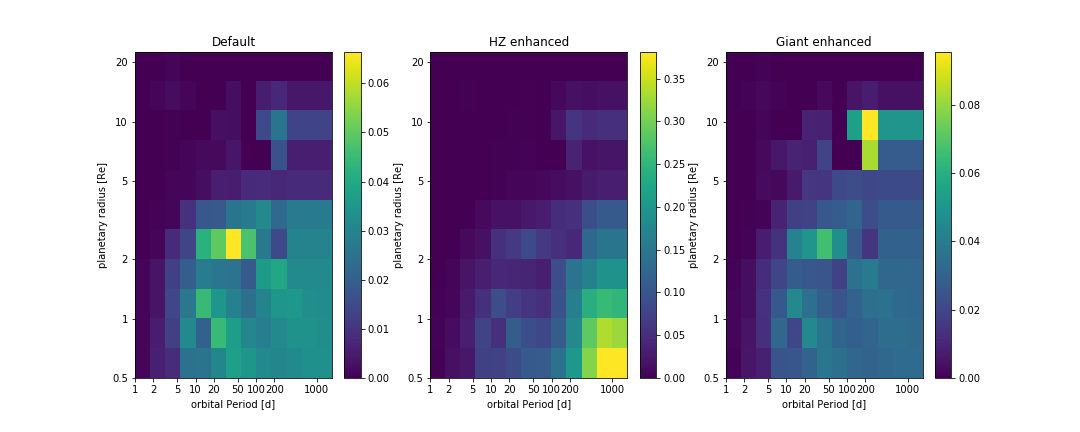
\includegraphics[width=\textwidth]{petigura_old_new2.png}
    \caption{Input planetary occurrence rates. The left panel shows those numbers pulled from \citet{petigura2018california}. In the case where bins are empty (e.g. long-period and small planets), an average of the nearest measured values are used.
    The central panel shows an adjusted input occurrence rate with more habitable planets (increased by a factor of between 1 and 10). The right panel shows an input occurrence rate for the background transiting planet (BTP) population with higher numbers of giant planets (increased by a factor of between 1 and 5).}
    \label{fig:occ_rates}
\end{figure}

Planets were sampled by generating a $13\times11$ grid of uniform random numbers (one for each period/radius bin) for each of the input stars and creating a planet everywhere the random number was less than the per-bin occurrence rate.
For each injected planet, precise parameters were chosen randomly between the $\log{P}$ and $R_p$ bin limits.
Random $t_0$(transit epoch) was chosen between 0 and $P$, a random eccentricity was chosen using the eccentricity distribution of \citet{kipping2013parametrizing}, a random $\omega$(the argument of periasteron) was chosen between 0 and $\pi$, and a random $\cos{i}$ (cosine of the inclination) was chosen between -1 and 1.
We also made an effort to make sure the majority of multiplanet systems were aligned by, in 66\% of cases, re-sampling the inclination of outer planets to a normal distribution around the inclination of the inner-most world (with $\sigma=5.72^\circ$).

From these generated quantities we could calculate the semi-major axis and remove any systems with unstably-short orbits (e.g. $sma < 2R_s$).
Next, impact parameter, depth and duration were calculated using the formulations of \citet{seager2003unique}.
Finally, using the RMS in the star catalogue, a signal-to-noise ratio was calculated and those planetary systems where no planet reached the necessary threshold (set to $3\sigma$) were removed.

Once this has been performed, we have a catalogue of potential transiting planetary systems.
In the case where this outnumbers the number of targets we are trying to generate a population for, we randomly choose planetary systems to fill all target stars. Otherwise, the loop starts again and more planetary systems are generated in the same manner.

Once we have our target stars (and associated planetary systems), we can compute some more secondary parameters such as Mass \citep[using the Mass-Radius relation of][]{weiss2014mass} surface temperature, albedo, doppler beaming coefficient, secondary eclipse impact parameter, radius ratio and surface brightness ratio.
Then, for each planet, we generate a lightcurve using the eclipsing binary code \citet{maxted2016ellc}, and assemble the full lightcurve afterwards.
Then, if randomly selected, stellar variability is computed for the target star (see section \ref{var}).
The planetary and variability lightcurves are then combined, interpolated to save space, and finally saved as delta magnitudes in a text file.


\subsection{Background transiting planets}
Background transiting planets were processed in much the same way as TPs, with three important differences.

First, rather than simple choosing a parent star from the "wide" target list, we instead select a single target star from that list and then randomly select a star from the "deep" catalogue of blends which is between 0 and 6 magnitudes fainter than the target star to be our planet host. For the new star we also have to recompute the total magnitude and RMS (for both star's light combined), as well as the amouth of dilution on the transit depth. This enables us to compute a SNR of the transits and reject any BTPs with SNR less than a threshold.

Unlike for TPs, we also take only the highest-SNR planet per system (as giant planets, the dominant source of BTP blends, are far more likely to be in single systems). 

Also, in order to boost the numbers of giant planets which form the dominant BTP false positives, we modified the input planet distribution to boost planets with radii between 5 and $13R_\oplus$ in all period bins (see Figure \ref{fig:occ_rates}).

Once a list of BTP systems has been generated, we again choose from that list the number of field positions we have selected to contain a BTP class and generate secondary information for each planet.
In the case of a blend, we also draw a random separation and angle between the brighter target star and the blended background star.
We do this by uniformly choosing a squared separation (which is uniform in area) between 0 and either the aperture radius \citep[derived with info from][]{marchiori2019flight} or 7 pixels (the limit around each star); whichever is smallest.
This allows a new RA and Dec to be computed for the injected background star.
Once again, a transit lightcurve is computed with \texttt{ellc} and, if randomly selected, stellar variability is also added before the lightcurve is interpolated and saved.
We also perform this step to add stellar variability (in 50\% of cases) to the brighter target star.


\subsection{Eclipsing Binaries}
Once again target stars are selected from the Besan\c{c}on “wide” catalogue. Rather than using occurrence rates from period and radius bins, we follow the results of \citet{raghavan2010survey} and select a uniform mass between 10 and 100% the mass of the primary target. Similarly we draw a period from a normal distribution in log period space around $5.03\pm2.28$ ($152.9^{+1342}_{-137.3}$d).
For the period and the masses oif both components, semi-major axis is calculated. Like for planets, $t_0$(eclipse time) is randomly sampled between 0 and $P$, $\omega$ from $0$ to $\pi$ and $\cos{i}$ from $-1$ to $1$.
To produce an eccentricity, we produce an adaptable beta distribution which varies as a function of period to mimic the distribution seen in Figure 6 of \citet{raghavan2010survey} (see Fig \ref{fig:EBecc}). 
We also set an uppoer bound to short-period EBs to match that seen in raghavan by setting the eccentricity of all EBs where $e>0.5*\log_10{P+10}$ to $0.0$.

\begin{figure}
    \centering
    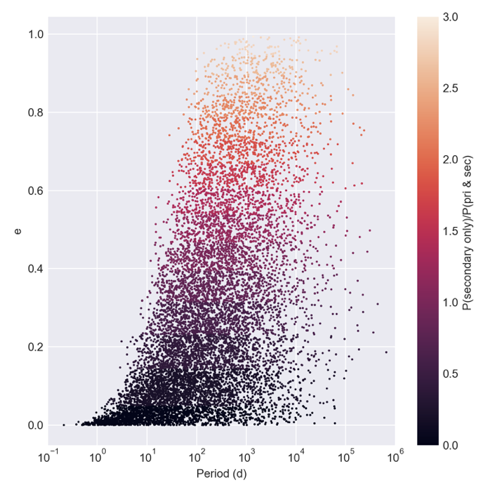
\includegraphics[width=\textwidth]{raghavan_Peccs.png}
    \caption{Period-eccentricity space modified from \citet{raghavan2010survey}.}
    \label{fig:EBecc}
\end{figure}

The next major difference is that, in order to understand the binary object injected, we must take the randomly generated secondary mass, plus parameters taken from the primary such as age and metallicity, to estimate a radius.
To do this requires isochrones. We use Dartmouth isochrones as implemented by \citet{morton2015isochrones}. 
These match best the distribution of stellar parameters as generated by the Besan\c{c}on models, however this comparison sometimes fails creating more evolved (e.g. larger-radius) secondaries than their primary companions - an unlikely situation for main sequence stars.
Therefore we cut there systems from the EB list.
We also, as for the planets, cut unstable systems where the semi-major axis is less than $1.5(R_1+R_2)$.

Next we calculate the impact factor of both primary and secondary eclipse, and remove non-eclipsing systems.
As EB companions around target stars are almost certainly high-SNR events, we make no attempt to derive and cut SNRs for this sample, and choose our necessary stars from this list.
Once these have been chosen, the durations, depths and SNRs of both primary and secondary eclipse are calculated.
We also compute extra stellar parameters such as limb darkening, gravity darkening, beaming coefficient, albedo, etc.

Finally \texttt{ellc} is used to generate lightcurves of the binary eclipses, and \texttt{celerite} is used to generate stellar variability (if specified). 

\subsection{Background Eclipsing Binaries}

The process for BEBs mirrors those described above for BTPs and EBs.
Once again target-blend pairs are randomly chosen, although in this case blend stars from Pmag to ${\rm Pmag}+10$ are used.
Masses, periods, eccentricities, etc are generates as for EBs.
Isochrones are  again used to generate the radius of the secondary, although it is the stellar information of the blended star which is used as the primary.
Again secondaries badly fitted by isochrones or with unstable orbits are removed. As are, once impact parameters are computed, binaries which do not produce primary or secondary eclipses.

In the case of BEBs, we perform cuts by SNR in order to make sure the input sample are all “detectable” by PLATO. 
To do this, it is important we recompute the PLATO-bandpass magnitude (and RMS) of all three stars together, and compute the dilution of the blended pair with respect to the target.
We must also compute primary and secondary duration and depth.
At this stage, the secondary stellar parameters are also computed.

Then, after targets with undetectable SNRs (<3.0 in the default) are removed, the requisite BEBs are selected to fill the open places in the fieldstars catalogue.

Once again, as with BTPs, a random separation and angle are sampled in order to compute a new RA and Dec.
Next interpolated lightcurves are generated for the background EB and, if variability is activated, for the target star.

\subsection{Stars without astrophysical signals}
For stars selected to have no astrophysical signal, a star is randomly selected from the input stellar catalogue.
A subsample of these (50\% in the default) are given stellar variability which is interpolated and saved to file.

\subsection{Stellar variability}\label{var}
To generate stellar variability, we wanted to mimic the effects of both Oscillations (which for G and F-type stars can be important).
To do this we loaded the \texttt{shocksgo} package which uses the damped simple harmonic motion (SHM) kernels of \texttt{celerite} to mimic the action of an asteroseismic osscilator \citep{foreman2018scalable}.
The \texttt{shocksgo} generates solar-like p-mode osscillations given input parameters such as temperature, density and radius. 

We also wanted to generate realistic activity given the imput. To do this we again used \texttt{celerite} but with a quasi-periodic to mimic the presence of transient spots on the stellar surface. This relies on three hyper-parameters - the persistence of individual signals (e.g. the damping parameter Q), the amplitude of vairability (A), and the frequency of the variation (i.e. the stellar rotation rate).
For each of these, we generated code to produce realistic distributions of these parameters. For example, for rotation period, we used the Age-Temperature relation of \citet{angus} to estimate a rotation rate for each input star.
For amplitude we generated a sampling method to roughly match the results seen in Kepler stars and presented by \citet{mcquillan2014rotation}. 
Although signal persistence (e.g. Q) has not been directely modelled, we used a normal distribution which peaked at  hot (e.g. A-type stars), albeit with larger scatter for high-mass stars.

\subsection{Blended stars}

\section{PlatoSim3 targets}


\subsection{Blended stars}

\section{PlatoSim3 targets}

\section{Installation}
First, a virtual environment, either with venv or conda, is probably necessary.

Second, PlatoSim3 should be installed, specially with the "develop" branch which allows photometric extraction. Details for installing PlatoSim3 from git can be found at \url{http://ivs-kuleuven.github.io/PlatoSim3/DownloadUpdateBuild.html}.

Clone the directory: \texttt{git clone https://github.com/hposborn/PlatoSim\_FieldGen}.

Next, pip install the requirements file: \texttt{pip install -t requirements.txt}.

There may be some special treatment here (e.g. to install the development version of \texttt{shocksgo} and an old version of \texttt{isochrones}).

\bibliographystyle{rusnat}
\bibliography{bib}

\end{document}
